%%%%%%%%%%%%%%%%%%%%%%%%%%%%%%%%%%%%%%%%%%%%%%%%%%%%%%%%%%%%%%%%%%%%%%%%%%%%%
% Paper F. The Settled-Gate Spacecraft FTC Benchmark.
% A short artifact/protocol note for arXiv (cs.RO / eess.SY) accompanying the
% released benchmark package (benchmark/BENCHMARK.md + leaderboard). The leaderboard
% tables are the SAME committed, evidence-generated tables used by Paper C
% (tables/), \input here verbatim so the note and the controller
% study can never disagree. No number in this note is authored by hand.
%%%%%%%%%%%%%%%%%%%%%%%%%%%%%%%%%%%%%%%%%%%%%%%%%%%%%%%%%%%%%%%%%%%%%%%%%%%%%
\documentclass[11pt]{article}
\usepackage[margin=1in]{geometry}
\usepackage{amsmath,amssymb}
\usepackage{graphicx}
\usepackage{booktabs}
\usepackage[hidelinks]{hyperref}
\usepackage{enumitem}
\usepackage{listings}
\lstset{basicstyle=\ttfamily\footnotesize,breaklines=true,columns=fullflexible,
  xleftmargin=1em,frame=none,showstringspaces=false}

\title{\textbf{The Settled-Gate Spacecraft Fault-Tolerant-Control Benchmark:\\
An Honest Protocol for Comparable Learned and Classical FTC}}
\author{Alireza Shojaei\\ \small Myers-Lawson School of Construction, Virginia Tech \quad \texttt{shojaei@vt.edu}}
\date{\today}

\begin{document}
\maketitle

\begin{abstract}
Recent learned fault-tolerant control (FTC) of spacecraft attitude is reported almost entirely in
simulation, on author-chosen fault sets, and against a \emph{transient-minimum} success criterion
that a trajectory need only touch once. On the same controllers, that criterion reads $\sim$$94\%$
where an honest steady-state gate reads $\sim$$60\%$, and the gap is limit-cycling that a touch-once
metric hides. We release a reproducible benchmark that closes this gap and gives the subfield a
single shared standard of evidence. A controller \emph{settles} a fault when its pointing error is
held within $0.2^\circ$ over a final-dwell window, scored on the \emph{true} simulator state and
never on a corrupted measurement. Faults are drawn from a \emph{structurally held-out} taxonomy over
inertia, gain magnitude, sign pattern, and additive bias, so a high score is generalization rather
than an i.i.d.\ resample of training. Each cell is $500$ episodes with Wilson $95\%$ confidence
intervals, and the environment is a pinned, pip-installable 6-DOF Basilisk simulator. We supply an
audited evaluation harness so that any policy is a drop-in, together with a reference leaderboard
spanning fault-unaware, classical-adaptive, two literature adaptive laws, end-to-end RL, and a
structured estimate-then-control design. The gate exposes one finding starkly. Constant additive
actuator bias (GAIN+BIAS) is recovered by no classical, learned, or RL controller, and not by a
privileged gain oracle either, because an integral-free law cannot null a constant bias; only a
disturbance-observer-augmented design recovers it ($59.4\%$). We release the benchmark so that future
FTC results are comparable and the gate is shared.
\end{abstract}

\section{Why the subfield needs a shared honest gate}
A spacecraft that loses, reverses, or degrades an actuator must recover its own pointing between
sparse ground contacts, often on the order of one short pass per orbit and sometimes far less when a
deep-space asset competes for a saturated Deep Space Network~\cite{OIG2023DSN}. The recovered state
that matters operationally is not a fleeting dip toward the target during a transient; it is a
\emph{held} attitude that science instruments, communication antennas, and momentum management can
all rely on for the remainder of the contact gap. Fault-tolerant attitude control is therefore a
crowded and well-motivated subfield, and learned methods have entered it in force. Yet the field's
empirical claims are difficult to compare against one another, and difficult to trust as predictors
of held-state recovery, because the community has not converged on a common standard of evidence.

A reading of the 2024--26 learned-FTC literature surfaces three recurring evaluation habits that, in
combination, inflate reported success and frustrate comparison. First, results are
\emph{sim-only}, which is appropriate for early-stage research but is rarely paired with a clearly
pinned and reinstallable environment, so a number reported in one paper cannot be regenerated under
another. Second, the fault set is \emph{author-chosen} and frequently overlaps the training
distribution, so a high score can be an in-distribution resample rather than evidence of
generalization to the off-nominal regimes a real failure produces. Transformer- and
distillation-based FTC for fixed-wing and rotary platforms, for instance, is typically demonstrated
on fault magnitudes inside the adaptation envelope it was trained over~\cite{Giral2024,Kim2025}.
Third, and most consequentially, ``recovery'' is scored as a \emph{transient minimum}, the pointing
error dipping below a threshold at some instant rather than holding a steady state. A controller can
satisfy a transient-minimum gate while limit-cycling indefinitely and never actually pointing, which
is precisely the failure an operator cannot tolerate.

These habits are not malpractice; they are the natural local optima of a subfield without a shared
gate, where each paper picks the metric, fault set, and testbed that best exhibit its own method. The
cost is collective. Numbers are not comparable across papers, headline success rates systematically
overstate held-state recovery, and the genuinely hard fault classes, the ones that separate a
controller that recovers from one that merely grazes, are obscured rather than surfaced. The remedy
is not a better single method but a better shared standard, a gate the whole subfield can adopt, on
which an honest number is lower but means what it says.

\subsection{Empirical case for the gate} The choice of gate materially changes the standings, and its effect
is large and measurable. On the identical controllers and faults of Table~\ref{tab:battery}, a
transient-minimum gate reports $\sim$$94\%$ success while the settled gate of this benchmark reports
$\sim$$60\%$. The $\sim$$34$-point gap is not noise and not a tuning artifact; it is steady-state
limit-cycling, in which the controller touches the target once and then oscillates, behavior the
touch-once metric scores as a clean success and the settled gate, correctly, does not. A gap of this
size on unchanged controllers is the quantitative case for the standard. A benchmark that does not
hold the controller to a dwell cannot distinguish recovery from a graze, and any leaderboard built on
such a metric ranks controllers by a quantity an operator does not care about. The settled gate is
the rigorous default the subfield needs, and the size of the gap is the measure of how much an easier
gate has been hiding.

\section{The protocol}
The benchmark fixes four design decisions, each chosen to make a reported number both honest and
comparable. We state each decision with its rationale, because a standard is only as useful as the
reasons others have to adopt it.

\subsection{The settled, steady-state gate} A controller \emph{settles} a fault when the pointing
error stays within $\mathbf{0.2^\circ}$ (the science-pointing requirement) over the \textbf{final dwell
window} ($20$ steps $=10$\,s), evaluated on the \textbf{true} simulator state rather than at a
transient minimum the trajectory touches once, and never on a corrupted measurement. The dwell is
what separates a held attitude from a graze, and it is the property an operator actually requires,
since an instrument integrates over the window rather than at the single best instant. Scoring on the
true state, not the measurement, is what keeps a sensor fault from being trivially ``passed'' by a
controller that has merely been fooled into reporting success. An \emph{operational} gate ($\leq 5^\circ$ held)
is reported alongside, so that a controller which stabilizes coarsely but misses the science
threshold is visibly distinguished from one that diverges. Each cell is $n{=}50$ held-out faults
$\times\,10$ seeds $=\mathbf{500}$ episodes.

\subsection{Wilson confidence intervals} A success rate over $500$ binary episodes is a binomial
proportion, and at the extremes that dominate an FTC leaderboard, near $0\%$ and near $100\%$, the
familiar normal-approximation (Wald) interval is badly miscalibrated and can even extend past
$[0,1]$. The Wilson score interval~\cite{Wilson} is the appropriate small-and-skewed-proportion
estimator, remains inside $[0,1]$, and does not collapse to zero width at a perfect cell. Reporting
the Wilson $95\%$ interval on every cell makes the leaderboard's uncertainty explicit and prevents a
one-episode difference between two near-perfect controllers from being read as a real separation.
Calibrated interval reporting of this kind is now standard practice in adjacent
machine-learning-with-guarantees work~\cite{Angelopoulos2023}, and an FTC benchmark should be held to
the same bar.

\subsection{Structurally held-out faults} The fault model is
$\tau_{\mathrm{applied}} = g\odot\tau_{\mathrm{cmd}} + b$ with body inertia scaled by $f$, applied to
the command inside the loop. Faults are split so the TEST set lives in regions of
$(f,|g|,\text{sign},b)$ the controller never trains on (Table~\ref{tab:split}). This is a deliberately
stronger condition than the usual i.i.d.\ train/test resample. The test faults are not merely unseen
samples from the training distribution, they lie \emph{outside its support} on every axis, so a high
TEST score is genuine extrapolative generalization rather than memorization or interpolation. A fault
is, by its nature, an off-nominal event, so a benchmark that only ever tests inside the nominal
envelope measures the wrong thing. The actuator classes are \textsc{sign} ($g\in\{\pm1\}$),
\textsc{gain} (continuous $g$), \textsc{gain+bias} ($g$ plus a constant bias $b$), and
\textsc{total\_loss} (one axis $g{=}0$, uncontrollable and so shield-only). The sensor classes, scored
on the true state through an observation corruptor, are a constant attitude bias, star-tracker
dropout, and a stuck measurement.

\begin{table}[h]\centering\small
\caption{Structurally held-out split. TEST faults lie outside the training support on every axis,
so a high TEST score cannot be an i.i.d.\ resample of training.}
\label{tab:split}
\begin{tabular}{lll}
\toprule
Axis & TRAIN & TEST (held out) \\
\midrule
Inertia scale $f$    & $[0.8, 2.0]$       & $[0.7,0.8)\cup(2.0,2.3]$ \\
Gain magnitude $|g|$ & $[0.5, 1.5]$       & $[0.3,0.5)\cup(1.5,2.0]$ \\
Sign pattern         & $\leq 1$ reversed axis & $\geq 2$ reversed axes \\
Additive bias $b$    & $[-0.2, 0.2]$      & $[-0.3,-0.2)\cup(0.2,0.3]$ \\
\bottomrule
\end{tabular}
\end{table}

\subsection{A pinned, reinstallable environment} \begin{sloppypar}A 6-DOF Basilisk attitude
simulator~\cite{Basilisk} is installed as a prebuilt wheel (\texttt{pip install bsk};
\texttt{import Basilisk}, v2.10.2), so that the testbed any submitter runs is byte-for-byte the
testbed the reference numbers were produced on. Attitude is in modified-Rodrigues-parameter (MRP)
coordinates~\cite{Schaub2018}, the observation is $[\sigma(3),\omega(3)]\in\mathbb{R}^6$, and the
action is three normalized torque commands $\in[-1,1]^3$. The timestep is $0.5$\,s, an episode is
$400$ steps ($200$\,s), the inertia is $\mathrm{diag}(10,8,6)$\,kg$\cdot$m$^2$, the max torque is
$0.2$\,N$\cdot$m, the nominal PD gains are $(k_p,k_d){=}(0.2,1.5)$, and the settled gate is
$0.2^\circ$ over the final $20$ steps. Pinning the version and shipping the wheel is what turns a
reported number from a claim into a fact a reader can independently reproduce; a benchmark whose
environment drifts between installs cannot anchor a leaderboard.\end{sloppypar}

\subsection{The evaluation harness} A controller is a fresh-per-episode policy
$\pi(\mathrm{obs})\!\to\!a\in[-1,1]^3$. The harness owns the parts of the experiment a submitter must
not be free to vary, namely it applies the fault to the command inside the loop, advances the pinned
simulator, scores the settled gate on the true state, and computes the Wilson interval over the
canonical $500$-episode battery. The submitter supplies only the policy. This separation is the point
of the harness design, since the most common way a benchmark number becomes incomparable is that two
authors silently differ on the gate, the fault battery, or the scoring side, and the harness removes
exactly those degrees of freedom.
\begin{lstlisting}
from program import rollout, eval_harness
from program.fault_taxonomy import FaultClass, heldout_test_faults

def my_maker(fault):        # fresh policy per (fault, seed), state resets
    return lambda obs: ...  # your controller
faults = heldout_test_faults(FaultClass.GAIN, n=50, seed=7000)  # TEST battery
res = eval_harness.evaluate(
    rollout.make_rollout_fn(my_maker), faults, list(range(10)))
print(res["settled_science"]["rate"],
      res["settled_science"]["wilson95"])
\end{lstlisting}
Sensor-fault evaluation passes a \texttt{make\_obs\_corruptor}. Tune only on TRAIN, and report the
settled gate and Wilson CIs on the canonical TEST battery. Submit an entry as a pull request adding
a producer plus its evidence JSON, with every leaderboard number re-derivable by re-running and
comparing to the committed value.

\section{Related work}
\subsection{Fault-tolerant attitude control} The classical foundations of spacecraft attitude
dynamics and control are well established~\cite{Schaub2018,Wie2008}, and fault-tolerant variants have
a long lineage in adaptive and robust control~\cite{IoannouSun1996}. The discrete control-direction
problem, in which an actuator's sign is unknown or reversed, is classically addressed by
Nussbaum-gain methods~\cite{Nussbaum1983}, with attitude-specific treatments handling actuator
saturation~\cite{Hu2018}. These methods are theoretically grounded and we include faithful
implementations as baselines, but they are typically validated by Lyapunov argument and a small set
of illustrative simulations rather than by a held-out statistical battery, so their behavior across a
broad off-nominal fault distribution and a steady-state gate has not been systematically reported.

\subsection{Learned FTC and its evaluation habits} A recent and fast-growing line applies learned
adaptation to FTC. Estimate-then-control designs infer a latent fault parameter online and feed
an analytic law, in the lineage of Neural-Fly~\cite{OConnell2022} and Rapid Motor
Adaptation~\cite{Kumar2021}, and transformer- or distillation-based controllers for rotary- and
fixed-wing platforms~\cite{Kim2025,Giral2024}. This work is genuinely capable, but it inherits the
three evaluation habits described in Section~1, since it is reported in simulation, on fault sets
that overlap the adaptation envelope, and against transient or episode-averaged criteria rather than
a held steady state. To our knowledge, RMA-style FTC has not been evaluated on spacecraft attitude
across a structurally held-out fault taxonomy with a settled gate, which is the gap this benchmark is
built to close. End-to-end reinforcement learning~\cite{SuttonBarto2018} is a natural alternative
hypothesis, and we include a from-scratch recurrent policy precisely so the benchmark can test
whether learning \emph{capacity}, absent estimate-then-control structure, suffices.

\subsection{Benchmarking and reproducibility as a methodology} The broader lesson that a subfield's
progress is gated by the quality of its shared evaluation, and that a rigorous, regenerable benchmark
with a pinned environment and a precise scoring rule is itself a contribution, is by now standard in
machine learning. Rigorous benchmarks that fix the task, the data, and the metric so that reported
numbers are comparable and reproducible have repeatedly reset expectations in their
fields~\cite{Zuo2025}, and calibrated-uncertainty reporting has become an expected
companion~\cite{Angelopoulos2023}. The contribution here is to bring that same discipline, a pinned
testbed, a precise and operationally meaningful gate, structurally held-out evaluation, interval
reporting, and one-command reproduction, to learned spacecraft FTC, where it has been largely absent.

\section{Reference leaderboard}
Table~\ref{tab:battery} (actuators) and Table~\ref{tab:sensor} (sensors) are the reference results
for this project, generated directly from the committed evidence. They are the identical tables used
by the companion controller study, \texttt{\textbackslash input} here verbatim so the benchmark note
and the study can never disagree. The leaderboard's purpose is not to crown a winner but to
demonstrate that the gate is discriminating. On an easy metric the rows would compress toward the
top and the table would say little, whereas on the settled gate the rows spread out and the genuinely
hard classes declare themselves (Fig.~\ref{fig:leaderboard}).

\begin{figure}[h]\centering
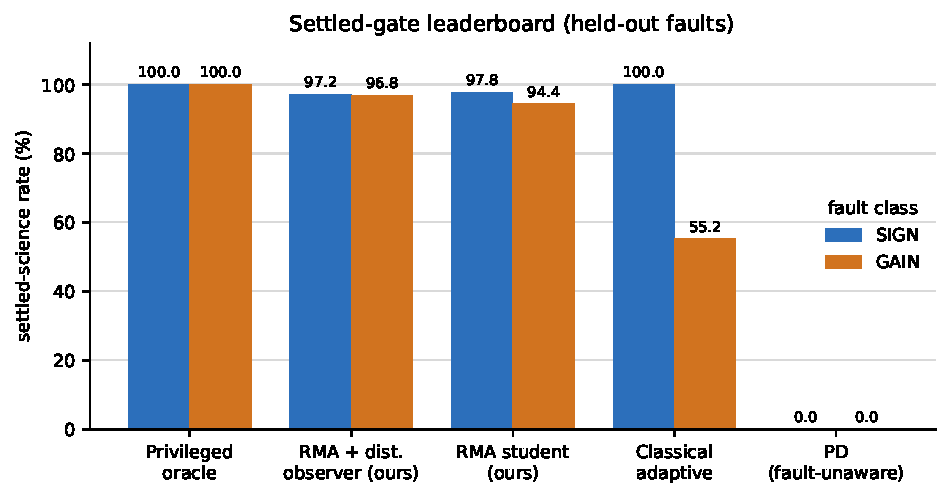
\includegraphics[width=0.82\linewidth]{figs/fig_leaderboard.pdf}
\caption{Headline standings on the two controllable continuous fault classes, ordered best
to worst by combined settled-science rate. The settled gate spreads the controllers across the
full range. The fault-unaware PD settles neither class, the classical adaptive law recovers
\textsc{sign} but degrades on \textsc{gain}, and the RMA student approaches the privileged
oracle on both. Every value is read from the same committed evidence as
Table~\ref{tab:battery}.}
\label{fig:leaderboard}
\end{figure}

% AUTO-GENERATED by evaluation.paper_c_controller_table.py
% from taxonomy_settled.json (WS1 battery) + gain_bias_dob.json (DOB).
\begin{table}[h]\centering\small
\caption{Definitive controller battery, reporting settled-science rate ($\leq0.2^\circ$ held over the final dwell) on the four structurally held-out fault classes ($n{=}500$/cell, same faults and gate across rows). \textbf{GAIN+BIAS is 0\% for every classical, learned, and RMA controller, and for the privileged gain oracle, which is the integral-free architectural limit; the RMA student composed with the disturbance observer is the only deployable controller to recover it}, with no SIGN/GAIN regression. A dead axis (LOSS) is uncontrollable (shield-only) for all.}
\label{tab:battery}
\begin{tabular}{lcccc}
\toprule
Controller & SIGN & GAIN & GAIN+BIAS & LOSS \\
\midrule
PD (fault-unaware) & 0.0\% & 0.0\% & 0.0\% & 0.0\% \\
Classical adaptive (sign-ID) & 100.0\% & 55.2\% & 0.0\% & 0.0\% \\
ICL-adaptive [lit.] & 82.2\% & 38.2\% & 0.0\% & 0.0\% \\
Nussbaum-gain [lit.] & 45.2\% & 3.2\% & 0.0\% & 0.0\% \\
End-to-end GRU+PPO & 0.0\% & 0.0\% & 0.0\% & 0.0\% \\
\midrule
RMA student, latched [WS1] & 97.8\% & 94.4\% & 0.0\% & 0.0\% \\
\textbf{RMA + disturbance obs.\ [ours]} & \textbf{97.2\%} & \textbf{96.8\%} & \textbf{59.4\%} & 0.0\% \\
\midrule
Privileged teacher (gain oracle) & 100.0\% & 100.0\% & 0.0\% & 0.0\% \\
Bias-feedforward oracle (g+b) & 100.0\% & 100.0\% & 95.8\% & 0.0\% \\
\bottomrule
\end{tabular}
\end{table}


The leaderboard makes one finding unmissable that an easier gate would bury. \textbf{Constant
additive actuator bias is $0\%$ for every classical, learned, and end-to-end controller, and for the
privileged gain oracle.} This is not a tuning failure but a structural one, and the benchmark is what
makes it visible. An estimate-then-control law that infers the gain but applies an integral-free
control cannot null a constant torque bias, since dividing the bias term by the gain estimate leaves
a residual that no amount of gain accuracy removes; the privileged gain oracle, which knows the true
gain exactly, therefore also sits at $0\%$. That the oracle fails alongside every learned and
classical method localizes the difficulty to the control architecture rather than to estimation
quality. Only the structured design augmented with a \emph{disturbance observer}, which recovers the
constant bias from the rigid-body dynamics and is self-correcting for gain-estimate
error~\cite{Chen2016}, recovers the class ($59.4\%$, against a bias-feedforward upper bound of
$95.8\%$), with no regression on \textsc{sign} or \textsc{gain}. A dead axis (\textsc{loss}) is
uncontrollable for all controllers and is the runtime shield's responsibility, not the controller's.
A leaderboard scored on a transient minimum would have reported this entire column near the top and
hidden the one architectural fact most worth knowing.

% AUTO-GENERATED by evaluation.paper_c_controller_table.py from sensor_faults.json
\begin{table}[h]\centering\small
\caption{Sensor-fault regimes (deployed RMA, settled gate, scored on the TRUE state). A constant attitude bias is controllable within the $0.2^\circ$ gate and offsets to exactly $-$bias beyond it (the sensor-side analog of actuator GAIN+BIAS); a lost or stuck attitude sensor removes position feedback (shield-only, the analog of TOTAL\_LOSS). The privileged teacher matches the controller on every row, so these are fundamental sensor-regime limits, and a sensor bias is unobservable from the corrupted measurement alone (unlike the actuator bias).}
\label{tab:sensor}
\begin{tabular}{lccl}
\toprule
Sensor fault & settled-science & final pointing & regime \\
\midrule
Sensor bias $0.1^\circ$ & 96.4\% & 0.10$^\circ$ & controllable \\
Sensor bias $0.2^\circ$ & 45.2\% & 0.20$^\circ$ & controllable \\
Sensor bias $0.3^\circ$ & 0.0\% & 0.30$^\circ$ & shield-only \\
Sensor bias $0.5^\circ$ & 0.0\% & 0.50$^\circ$ & shield-only \\
Star-tracker dropout & 0.0\% & 97.19$^\circ$ & shield-only \\
Stuck measurement & 0.0\% & 85.56$^\circ$ & shield-only \\
\bottomrule
\end{tabular}
\end{table}


The sensor side is classified the same way and exhibits the same controllable-versus-shield-only
boundary. A constant attitude-measurement bias is controllable within the gate and offsets to exactly
$-$bias beyond it, the sensor-side analog of the actuator GAIN+BIAS wall, and unlike the actuator bias
it is unobservable from the corrupted measurement alone, so it cannot be removed by a disturbance
observer. A lost or stuck attitude sensor removes position feedback entirely and is a shield-only
regime, the analog of \textsc{total\_loss}. That the privileged teacher matches the controller on
every sensor row indicates these are fundamental regime limits rather than controller deficiencies,
which is exactly the kind of distinction a steady-state gate scored on the true state is able to draw.

\section{Discussion}
A shared honest gate changes what the subfield can say. Once recovery means a held steady state on
faults outside the training support, scored on the true state with reported intervals, three things
follow that an easier metric prevents. First, numbers become comparable, and a $59.4\%$ on this gate
means the same thing in any paper that adopts it, so results accumulate into a leaderboard rather than
a collection of incomparable claims. Second, the hard classes surface instead of hiding. The
GAIN+BIAS wall is invisible to a transient-minimum metric and obvious here, and surfacing it is what
turned it from an unnoticed $0\%$ into a posed problem with a disturbance-observer answer; a standard
that hides its hardest cases cannot drive progress on them. Third, the burden of proof shifts in the
right direction. Under a shared gate a high number is a strong claim a reader can independently
reproduce from a clean checkout, rather than a figure contingent on an author's private metric and
testbed.

We expect the immediate effect of adopting the gate to be that some published successes read lower,
which is the intended correction rather than a defect. A $94\%$ that was really a $60\%$ was never a
property of the controller; it was a property of the metric, and replacing it with a number that
means held-state recovery is what lets the subfield trust its own leaderboard. The gate is deliberately
strict so that the easy way to a high score, optimizing the metric rather than the behavior, is closed
off. The contribution we are most committed to is therefore the gate and the harness, not any
particular leaderboard position; the position is evidence that the gate discriminates, and the gate is
the thing we are asking the subfield to share.

\subsection{Limitations and scope} The benchmark is single-environment and seed-controlled, which is
what makes it exactly reproducible but also means it is a protocol for comparable
\emph{simulation} evidence and a TRL-2-to-3 instrument, not a flight qualification. The actuator
model is external-torque injection rather than a full reaction-wheel-momentum model, a fidelity
upgrade we regard as the natural next version of the testbed rather than a change to the protocol. The
$0.2^\circ$ science gate, the $200$\,s horizon, and the fault-magnitude ranges are concrete and
defensible choices for the rigid-body regime modeled here, and a different mission class would
re-instantiate the same protocol with its own such constants; the protocol, not the particular
numbers, is the portable contribution. Finally, the leaderboard reported here is one project's
reference set, and the submission rule exists precisely so that the gate, once shared, is populated by
the community rather than by us.

\section{Release and reproduction}
The benchmark package (\texttt{benchmark/BENCHMARK.md} and the auto-generated leaderboard) pins the
gate, taxonomy, environment, harness, and submission rule. The leaderboard producers each write
verifiable evidence JSON, headline numbers are re-checked from a clean checkout by a single
reproduce script, and any single number is re-derivable with a verify-number utility that re-runs it
and compares to the committed value. We release the package so that every learned-FTC paper that
adopts the settled gate is directly comparable to every other. The gate, not the leaderboard
position, is the contribution.

\begin{thebibliography}{99}\small
\bibitem{Basilisk} P.~W.~Kenneally, S.~Piggott, H.~Schaub. ``Basilisk: a flexible, scalable and modular astrodynamics simulation framework.'' \emph{J.\ Aerospace Information Systems}, 17(9):496--507, 2020.
\bibitem{Wilson} E.~B.~Wilson. ``Probable inference, the law of succession, and statistical inference.'' \emph{J.\ Amer.\ Statist.\ Assoc.}, 22(158):209--212, 1927.
\bibitem{Schaub2018} H.~Schaub, J.~L.~Junkins. \emph{Analytical Mechanics of Space Systems}, 4th ed. AIAA Education Series, 2018.
\bibitem{Wie2008} B.~Wie. \emph{Space Vehicle Dynamics and Control}, 2nd ed. AIAA Education Series, 2008.
\bibitem{IoannouSun1996} P.~A.~Ioannou, J.~Sun. \emph{Robust Adaptive Control}. Prentice-Hall, 1996.
\bibitem{Nussbaum1983} R.~D.~Nussbaum. ``Some remarks on a conjecture in parameter adaptive control.'' \emph{Systems \& Control Letters}, 3(5):243--246, 1983.
\bibitem{Hu2018} Q.~Hu, X.~Shao, Y.~Zhang, L.~Guo. ``Nussbaum-type function-based attitude control of spacecraft with actuator saturation.'' \emph{Int.\ J.\ Robust and Nonlinear Control}, 28(8):2927--2949, 2018.
\bibitem{Chen2016} W.-H.~Chen, J.~Yang, L.~Guo, S.~Li. ``Disturbance-observer-based control and related methods, an overview.'' \emph{IEEE Trans.\ Industrial Electronics}, 63(2):1083--1095, 2016.
\bibitem{Kumar2021} A.~Kumar, Z.~Fu, D.~Pathak, J.~Malik. ``RMA: Rapid Motor Adaptation for legged robots.'' \emph{Robotics: Science and Systems (RSS)}, 2021.
\bibitem{OConnell2022} M.~O'Connell, G.~Shi, X.~Shi, K.~Azizzadenesheli, A.~Anandkumar, Y.~Yue, S.-J.~Chung. ``Neural-Fly enables rapid learning for agile flight in strong winds.'' \emph{Science Robotics}, 7(66):eabm6597, 2022.
\bibitem{Kim2025} D.~Kim, J.~D.~Lee, H.~Bang, J.~Bae. ``Reinforcement learning-based fault-tolerant control for quadrotor with online transformer adaptation.'' \emph{ICRA Workshop: Robots in the Wild}, 2025.
\bibitem{Giral2024} F.~Giral, I.~G\'omez, R.~Vinuesa, S.~Le~Clainche. ``Transformer-based fault-tolerant control for fixed-wing UAVs using knowledge distillation and in-context adaptation.'' arXiv:2411.02975, 2024.
\bibitem{SuttonBarto2018} R.~S.~Sutton, A.~G.~Barto. \emph{Reinforcement Learning: An Introduction}, 2nd ed. MIT Press, 2018.
\bibitem{Angelopoulos2023} A.~N.~Angelopoulos, S.~Bates. ``Conformal prediction: a gentle introduction.'' \emph{Found.\ Trends Mach.\ Learn.}, 16(4):494--591, 2023.
\bibitem{Zuo2025} M.~Zuo, F.~Piedrahita Velez, X.~Li, M.~L.~Littman, S.~H.~Bach. ``Planetarium: a rigorous benchmark for translating text to structured planning languages.'' \emph{NAACL}, 2025.
\bibitem{OIG2023DSN} NASA Office of Inspector General. ``NASA's management of the Deep Space Network.'' Report IG-23-016, 2023.
\end{thebibliography}

\end{document}
